% ============================================================
% IE UNIVERSITY - BACHELOR IN APPLIED MATHEMATICS
% MACHINE LEARNING & COMMUNICATION SKILLS PROJECT PROPOSAL
% ============================================================

\documentclass[clean]{bam-proposal}

\BAMtitle{Is Ranking Students by Raw GPA Fair Across Degrees?}
\BAMteam{Adam Bajer; Pablo Torres; Ignacio Gimeno}
\BAMcourse{Machine Learning \& Communication Skills}
\BAMacademicyear{2026--2027}
\BAMsubmissiondate{11 October 2026, 23:59 Madrid time}

\BAMbibliographystyle{amsplain}
\BAMbibliographyfile{references}

\begin{document}
\makeproposalheader

% ============================================================
\section{Problem, Motivation, and Research Question}

When a university has a limited number of places to give out, it often puts students from every degree on one list and sorts them by grade point average. IE University allocates exchange destinations like this. Applicants are ordered by credit-weighted GPA, and whoever ranks higher chooses a destination first. Under this rule an 8.0 in Business Administration counts the same as an 8.0 in Applied Mathematics, which is only reasonable if both degrees grade to the same standard. There are good reasons to doubt that. Studies of single institutions have found that departments grade systematically differently \cite{sabot1991grade,achen2009grades}, and a study of 33 US public universities found large gaps between departments that repeat from one university to the next \cite{jeong2024grades}. If Spain shows the same pattern, a student's place on a single GPA list depends in part on which degree they chose.

Our research question is: \emph{how much of a student's position in a university-wide GPA ranking is determined by the field of study, and how would ranking students within their degree change who is selected for a fixed number of places?} We answer it in three stages. Using data from all Spanish universities, we measure how much of the variation in graduates' grades the field explains once university and year are held fixed. With individual student records we then check whether the gap between degrees remains after controlling for entry grades, since weaker intakes in some degrees are the most likely alternative explanation. Last, we simulate a top-20\% selection with raw and with degree-normalised grades. The project measures differences in grading and makes no claim about how intrinsically difficult each degree is. We intend the results to be useful to universities, our own included, that are reviewing GPA-based selection rules.

% ============================================================
\section{Data and Exploratory Analysis}

The main source is the SIIU table of graduates' final grades published by the Spanish Ministry of Universities \cite{siiu2025}. One observation is a university, a field of study and an academic year, with the mean, the three quartiles and the maximum final grade on the 5--10 scale. After keeping the 29 detailed fields, dropping the aggregate categories and combining both sexes, we have 12,125 observations from 89 universities between 2015--16 and 2023--24. About half of the possible cells are empty, either because the Ministry suppresses small groups or because the university does not offer the field. The table is official and covers the whole Spanish system, IE University included, and the quartiles give us the spread within each field that the ranking simulation needs. Its weaknesses are that it is aggregated, that it only counts students who graduated, and that it groups degrees into broad fields.

The second source is the UCI dataset ``Predict Students' Dropout and Academic Success'' \cite{realinho2021uci,realinho2022data}. It holds 4,424 students of a Portuguese polytechnic, with their degree, admission grade, previous qualification grade, demographic variables and first-year results on the 0--20 scale. We compute first-year GPA as the average of the two semester means, weighted by the number of units passed in each. Students who passed no unit (676) have no GPA and are left out, and so are two degrees with too few usable records, which leaves 3,703 students in 15 degrees. Because the two sources have no common key we analyse them separately; each covers a part of the question the other cannot.

Figure~\ref{fig:eda} summarises the exploratory analysis of the Spanish data. In 2023--24 the median university mean goes from about 6.8 in Agriculture to 7.9 in Nursing, and within each field the universities are fairly close to one another. The ordering is not a split between STEM and the rest. Business Administration, Economics and Law are among the lowest-graded fields, and in the 34 universities that report both, Mathematics \& Statistics graduates average 0.25 points more than Business Administration graduates (standard error 0.035 across universities). IE University is above the national distribution in every field it reports: its field means lie between 8.01 and 8.52, while the national average is 7.41. In the Portuguese data the highest and lowest degree means are 1.51 points apart, more than the overall standard deviation of 1.27, and admission grade is only moderately correlated with GPA ($r = 0.31$).

\begin{figure}[htbp]
  \centering
  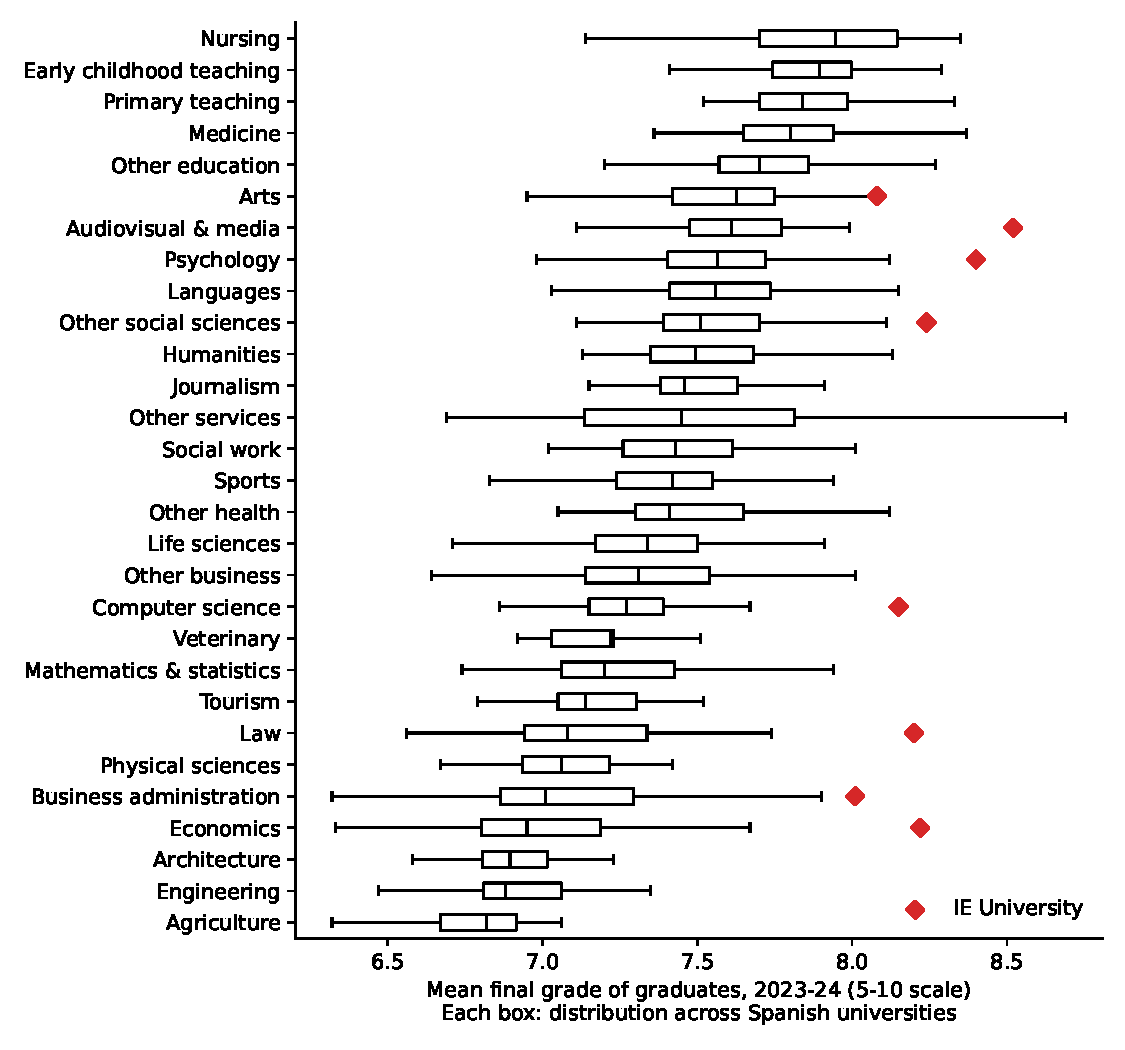
\includegraphics[width=0.74\linewidth]{figures/spain_grades_by_field.pdf}
  \caption{Graduates' mean final grade differs systematically by field of study. Each box shows the distribution of university-level means for one field across Spanish universities in 2023--24 (scale 5--10; whiskers at 1.5 IQR, outliers hidden). Red diamonds mark IE University. Source: SIIU \cite{siiu2025}; 29 detailed fields, both sexes.}
  \label{fig:eda}
\end{figure}

% ============================================================
\section{Preliminary Methodology and Results}

Our first model is a linear regression of each university-field-year mean on field indicators, with university and year fixed effects. We use sum coding, so each field effect is the distance from the average field. University and year on their own explain 18\% of the variance, and adding the field brings this to 70\% ($F = 739$ on 28 degrees of freedom). The field effects go from $-0.56$ for Architecture to $+0.55$ for Nursing, a spread of 1.1 points between fields of the same university in the same year.

A pattern that held only in a few large universities would be of little use, so we also test it on universities the model has not seen. The target is each field's deviation from its university-year average, and the model is a ridge regression on one-hot field indicators. We set aside 18 universities (20\%) as a test set and tune and validate on the other 71 with 10-fold cross-validation grouped by university, which keeps every university entirely inside one fold. As Table~\ref{tab:preliminary-results} shows, the field alone lowers the error from 0.353 to 0.221 in validation, and from 0.366 to 0.231 on the test universities.

The Portuguese records let us check whether entry grades explain the gap. Predicting every student at the mean gives an error of 1.255; a linear model with entry grades and background lowers it to 1.167, and adding the degree lowers it to 1.092. The held-out test students rank the models in the same order. In the full OLS model the gap between the highest and lowest degree falls from 1.51 to 1.31 points after these controls, and the degree effects stay jointly significant ($F = 37.9$ on 14 degrees of freedom; Figure~\ref{fig:portugal}). Entry grades account for only a small part of the difference between degrees.

\begin{table}[htbp]
  \centering
  \caption{Preliminary model performance, measured as root mean squared error (lower is better). Validation: mean $\pm$ standard deviation over 10 folds of the training data (grouped by university for Spain). Test: a single evaluation on held-out data never used for fitting or tuning (Spain: 18 universities, 2,559 observations; Portugal: 741 students, stratified by degree).}
  \label{tab:preliminary-results}
  \begin{tabularx}{0.92\linewidth}{@{}Xcc@{}}
    \toprule
    Model & Validation RMSE & Test RMSE \\
    \midrule
    \multicolumn{3}{@{}l}{\emph{Spain: field mean minus university-year average (grade points, 5--10 scale)}} \\
    Baseline: zero deviation (field ignored) & $0.353 \pm 0.033$ & 0.366 \\
    Ridge: field of study & $0.221 \pm 0.020$ & 0.231 \\
    \midrule
    \multicolumn{3}{@{}l}{\emph{Portugal: first-year GPA (grade points, 0--20 scale)}} \\
    Baseline: overall mean & $1.255 \pm 0.048$ & 1.313 \\
    Linear: entry grades and background & $1.167 \pm 0.053$ & 1.227 \\
    Ridge: entry grades, background and degree & $1.092 \pm 0.053$ & 1.168 \\
    \bottomrule
  \end{tabularx}
\end{table}

To see what these gaps mean for selection, we simulate a top-20\% cut in every university-year with at least four fields. Each field's grades are approximated by a normal distribution with the reported mean and a standard deviation equal to the interquartile range divided by 1.349; we pool the fields and find the cutoff that admits 20\% of graduates. Across 718 university-years (85 universities), 43\% of Nursing graduates end up inside their university's top 20\%, compared with 9\% in Business Administration and 6\% in Engineering (Figure~\ref{fig:selection}). In the Portuguese data, ranking by a within-degree z-score instead of raw GPA moves 138 of the 741 places (19\%) in a cut of the same size. So a raw-GPA list sorts students to a large extent by field. We do not yet say which normalisation is fairest, because each one assumes something about how able the students of each degree are.

\begin{figure}[htbp]
  \centering
  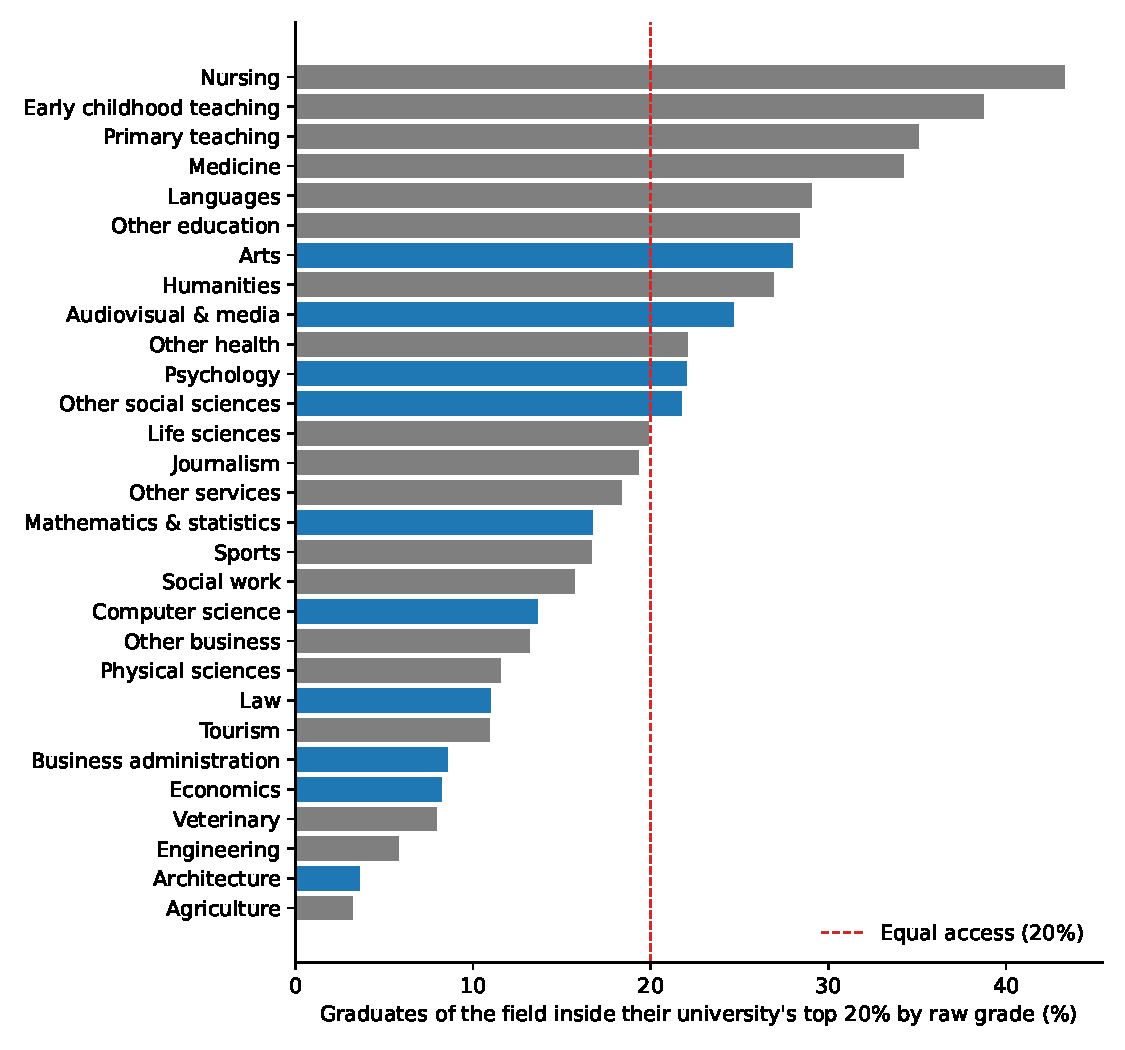
\includegraphics[width=0.74\linewidth]{figures/spain_selection_by_field.pdf}
  \caption{Under a single ranking by raw grade, access to a top-20\% cut depends strongly on the field. Bars show the average share of each field's graduates above their university's top-20\% cutoff, over 718 university-years from 85 Spanish universities (2015--16 to 2023--24). Within-field grades are approximated as normal from the reported mean and quartiles; fields are weighted equally. Blue bars are fields offered at IE University; the dashed line marks equal access. Source: SIIU \cite{siiu2025}.}
  \label{fig:selection}
\end{figure}

\begin{figure}[htbp]
  \centering
  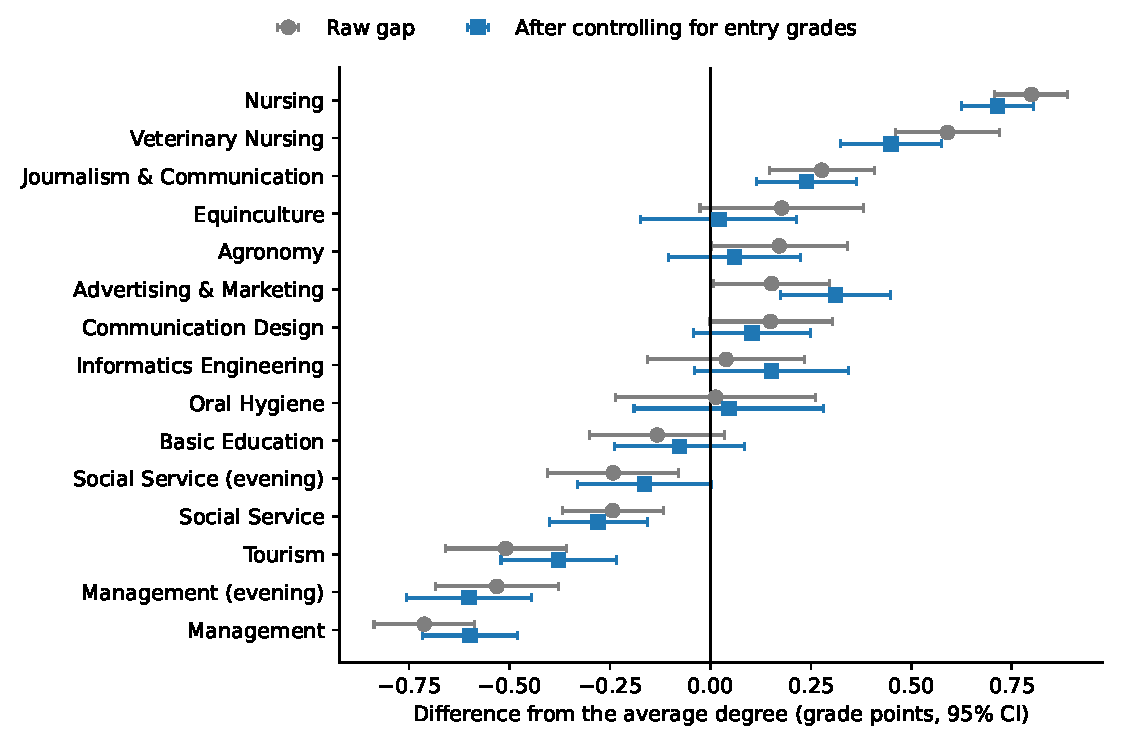
\includegraphics[width=0.74\linewidth]{figures/degree_effects.pdf}
  \caption{Degree effects on first-year GPA barely change after controlling for entry grades. Points show each degree's difference from the average degree (0--20 scale) with 95\% confidence intervals, from OLS without controls (grey) and with admission grade, previous qualification grade, age, sex, scholarship, displaced and international status (blue). Data: 3,703 students in 15 degrees of a Portuguese polytechnic \cite{realinho2021uci}.}
  \label{fig:portugal}
\end{figure}

% ============================================================
\section{Next Steps, Reproducibility, and Ownership}

Before the Progress Report we will, in this order: (1) weight the simulation by the number of graduates in each field, taken from the Ministry's enrolment tables, because equal weights give small fields too much influence; (2) fit a logistic regression for the probability of reaching the top 20\% given field and university, and compare it with the regression approach; (3) compare three normalisation rules (within-degree z-score, percentile and regression-adjusted GPA) and spell out what each assumes about student ability; (4) cluster fields by their grade profile (mean, quartiles and trend) using $k$-means on standardised features, and look at the clusters with PCA. If there is time, we will repeat the field-effect analysis on the 33-university US dataset \cite{jeong2024grades}. The largest risk is that aggregated data cannot tell grading standards apart from student ability. The Portuguese records address this only in part, and we will say so in the report.

The analysis is written in Python (pandas, statsmodels, scikit-learn) and will be developed in a public GitHub repository. Raw data stay unchanged. The scripts regenerate every figure, table and number in this proposal and write them to results files, random seeds are fixed at 42, and the package requirements are listed.

% ============================================================
\BAMprintbibliography

\section*{Declaration of Contributions and AI Use}

\textbf{Teamwork.} The three members chose the topic and the research question together. Ignacio Gimeno coordinated the project, ran the analysis and prepared and submitted the proposal. Adam Bajer and Pablo Torres reviewed the research question and the proposal.

\textbf{Generative AI.} Ignacio Gimeno used Claude (Anthropic) to locate data sources, to write the Python code for data cleaning, modelling, cross-validation and figures, and to draft and revise the wording of this proposal. The team checked every reported number against the outputs of the scripts, checked each reference against its DOI record or the publisher's page, and is responsible for all content.

\end{document}
